\subsection{Gaussian Elimination and Pivoting}



\frame{
\begin{block}{}
\begin{itemize}
\item In this section we develop a scheme for solving a general system $A X = B$ of $N$ equations and $N$ unknowns. 
\begin{center}
$\Downarrow$
\end{center}
\item The goal is to {\Large construct an equivalent upper-triangular system} $U X = Y$ that can be solved by the method of the back-substitution algorithm.
\end{itemize}
\end{block}
\vspace{3mm}
\begin{block}{}
\begin{itemize}
\item Two linear systems of dimension $N \times N$ are said to be equivalent provided that their solution sets are the same.  \\
\item Theorems from linear algebra show that when certain transformations are applied to a given system, the solution sets do not change.
\end{itemize}
\end{block}
}

\frame{
\begin{block}{Theorem (Elementary Transformations).} 
The following operations applied to a linear system yield an equivalent system:
\begin{description}
 \item [Interchanges :] The order of two equations can be changed.
 \item [Scaling :] Multiplying an equation by a nonzero constant.
 \item [Replacement :] An equation can be replaced by the sum of itself and a nonzero multiple of any other equation.
\end{description}
\end{block}
\vspace{5mm}
It is common to use the {\Large Replacement Elementary Transformation} by replacing an equation with the difference of that equation and a multiple of another equation. 
}

\frame{
\frametitle{Example.}
Find the parabola $y = A+ B x + C x^2$ that passes through the three points $(1, 1)$, $(2,-1)$, and $(3, 1)$.
\begin{center}
$\Downarrow$
\end{center}
For each point we obtain an equation relating the value of $x$ to the value of $y$. 
The result is the linear system
\begin{equation*}
\begin{array}{r r r c r l}
A  + &   B + &   C & = &    1 & at \ (1, 1)\\
A  + & 2B + & 4C & = & -1 & at \ (2,-1)\\
A  + & 3B + & 9C & = &   1 & at \ (3, 1).
\end{array}
\end{equation*}
\begin{center}
$\Downarrow$
\end{center}
The variable $A$ is eliminated from the second and third equations by subtracting the first equation from them. 
}

\frame{
This is an application of the replacement transformation, and the resulting equivalent linear system is
\begin{equation*}
\begin{array}{r r r c r }
A   + & B + &   C & = &   1 \\
         & B + & 3C & = & -2 \\
 & 2B + & 8C & = &   0
\end{array}
\end{equation*}
\begin{center}
$\Downarrow$
\end{center}
The variable $B$ is eliminated from the third equation by subtracting from it two times the second equation. 
We arrive at the equivalent upper-triangular system:
\begin{equation*}
\begin{array}{r r r c r }
A   + & B + &   C & = &   1 \\
         & B + & 3C & = & -2 \\
         &       & 2C & = &   4
\end{array}
\end{equation*}
}

\frame{
The {\Large back-substitution algorithm} is now used to find the coefficients:
\begin{equation*}
\begin{array}{c c c c r} 
C & = & 4/2 & = & 2  \\
B & = &  -2 - 3(2) & = & -8 \\ 
A & = & 1 - (-8) - 2 & = & 7 
\end{array}
\end{equation*}
and the equation of the parabola is
\begin{equation*}
y = 7 - 8x + 2x^2.
\end{equation*}
}

\frame{
\begin{block}{}
\begin{itemize}
\item It is efficient to store all the coefficients of the linear system $AX = B$ in an array of dimension $N \times (N + 1)$. 
\item The coefficients of $B$ are stored in column $N + 1$ of the array (i.e., $a_{kN+1} = b_k$). 
\item Each row contains all the coefficients necessary to represent an equation in the linear system. 
\item The {\Large augmented matrix} is denoted $[AlB]$ and the linear system is represented as following equation
\begin{equation*}
[A|B] = 
\left[ 
\begin{array}{l l l l | l}
a_{1,1} & a_{1,2} & \cdots & a_{1,N} & b_1 \\
a_{2,1} & a_{2,2} & \cdots & a_{2,N} & b_2 \\
\vdots & \vdots & \ddots & \vdots & \vdots \\
a_{N,1} & a_{N,2} & \cdots & a_{N,N} & b_N 
\end{array}
\right]
\end{equation*}
\end{itemize}
\end{block}
}

\frame{
\begin{block}{}
\begin{itemize}
\item The system $AX = B$,  can be solved by performing row operations on the augmented matrix $[AlB]$. 
\vspace{5mm}
\item The variables $X_k$ are placeholders for the coefficients and can be omitted until the end of the calculation.
\end{itemize}
\end{block}
}


\frame{
\begin{block}{Theorem  (Elementary Row Transformations).} 
The following operations applied to the augmented matrix yield an equivalent linear system:
\begin{description}
 \item [Interchanges :] The order of two equations can be changed.
 \item [Scaling :] Multiplying a row by a nonzero constant.
 \item [Replacement :] The row can be replaced by the sum of that row and a nonzero multiple of any other row; 
that is:
$ row_r = row_r - m_{rp} \times row_p.$
An equation can be replaced by the sum of itself and a nonzero multiple of any other equation.
\end{description}
\end{block}
\vspace{5mm}
It is common to use the {\Large Replacement Elementary Transformation} by replacing an equation with the difference of that row and a multiple of another row. 
}


\frame{
\begin{block}{Definition.} 
The number $a_{r, r}$ in the coefficient matrix $A$ that is used to eliminate $a_{k, r}$ , 
where $k = r + 1, r + 2, \ldots , N$, is called the $r$-th {\Large pivotal element}, and the $r$-th row is called the {\Large pivot row}.
\end{block}
\vspace{15mm}
The following example illustrates how to use the operations in above Theorem to obtain an equivalent upper-triangular system $ UX = Y$ from a linear system $AX = B$, where $A$ is an $N \times N$ matrix.
}

\frame{
\frametitle{Example (Gaussian elimination) }
Express the following system in augmented matrix form and find an equivalent upper-triangular system and the solution.
\begin{equation*}
\begin{array}{r c r c r c r c c}
    x_1 & + & 2x_2 & + &   x_3 & + & 4x_4 & = & 13 \\
  2x_1 & + & 0x_2 & + & 4x_3 & + & 3x_4 & = & 28 \\
  4x_1 & + & 2x_2 & + & 2x_3 & + &   x_4 & = & 20 \\
-3x_1 & + &   x_2 & + & 3x_3 & + & 2x_4 & = & 6
\end{array}
\end{equation*}
\begin{center}
$\Downarrow$
\end{center}
The augmented matrix is
\begin{equation*}
\begin{array}{r}
pivote \ \rightarrow \\
m_{21} = 2 \\
m_{31} = 4 \\
m_{41} = -3
\end{array}
\left[
\begin{array}{c c c c | c}
  \underline{1} & 2 & 1 & 4 & 13 \\
  2 & 0 & 4 & 3 & 28 \\
  4 & 2 & 2 & 1 & 20 \\
-3 & 1 & 3 & 2 & 6 
\end{array}
\right]
\end{equation*}
}

\frame{
\begin{itemize}
\item The first row is used to eliminate elements in the first column below the diagonal.
\item We refer to the first row as the {\Large pivotal row} and the element $a_{11} = 1$ is called the {\Large pivotal element}. 
\item The values $m_{k1}$ are the multiples of row $1$ that are to be subtracted from row $k$ for $k = 2, 3, 4$. 
\end{itemize}
The result after elimination is
\begin{equation*}
\begin{array}{r}
 \\
pivote \ \rightarrow \\
m_{32} = 1.5 \\
m_{42} = -1.75
\end{array}
\left[
\begin{array}{c c c c | c}
  1 & 2 & 1 & 4 & 13 \\
  0 & \underline{-4} & 2 & -5 & 2 \\
  0 & -6 & -2 & -15 & -32 \\
  0 & 7 & 6 & 14 & 45 
\end{array}
\right]
\end{equation*}
}

\frame{
\begin{itemize}
\item The second row is used to eliminate elements in the second column that lie below the diagonal. 
\item The second row is the pivotal row and the values $m_{k2}$ are the multiples of row $2$ that are to be subtracted from row $k$ for $k = 3, 4$. 
\end{itemize}
The result after elimination is
\begin{equation*}
\begin{array}{r}
 \\
 \\
pivote \ \rightarrow \\
m_{43} = -1.9
\end{array}
\left[
\begin{array}{c c c c | c}
  1 & 2   & 1 & 4 & 13 \\
  0 & -4 & 2 & -5 & 2 \\
  0 & 0   & \underline{-5} & -7.5 & -35 \\
  0 & 0   & 9.5 & 5.25 & 48.5 
\end{array}
\right]
\end{equation*}
}

\frame{
Finally, the multiple $m_{43} = -1.9$ of the third row is subtracted from the fourth row, and
 the result is the upper-triangular system
\begin{equation*}
\left[
\begin{array}{c c c c | c}
  1 & 2   & 1   & 4      & 13 \\
  0 & -4 & 2   & -5    & 2 \\
  0 & 0   & -5 & -7.5 & -35 \\
  0 & 0   & 0   & -9 & -18 
\end{array}
\right]
\end{equation*}
\begin{center}
$\Downarrow$
\end{center}
The {\Large back-substitution algorithm} can be used to solve above argument matrix, and we get
\begin{equation*}
\begin{array}{c c c}
x_4 & = & 2   \\
x_3 & = & 4   \\
x_2 & = & -1\\ 
x_1 & = & 3
\end{array}
\end{equation*}
}

\frame{
\begin{itemize}
\item The process described above is called {\Large Gaussian elimination} and must be modified so that it can be used in most circumstances. 
\item If $a_{kk} = 0$, row k cannot be used to eliminate the elements in column $k$, and row $k$ must be interchanged with some row below the diagonal to obtain a nonzero pivot element. 
\item If this cannot be done, then the coefficient matrix of the system of linear equations is singular, and the system does not have a unique solution. 
\end{itemize}
}

\frame{
\begin{block}{Theorem (Gaussian Elimination with Back Substitution).} 
If $A$ is an $N \times N$ nonsingular matrix, 
then there exists a system $U X = Y$, equivalent to $A X = B$, 
where $U$ is an upper-triangular matrix with $u_{k, k} = 0$.
After $U$ and $Y$ are constructed, back substitution can be used to solve $U X = Y$ for $X$.
\end{block}
Proof : \\
We will use the augmented matrix with $B$ stored in column $N + 1$
\begin{equation*}
A X = 
\left[
\begin{array}{c c c c c}
a_{1,1}^{(1)} & a_{1,2}^{(1)} & a_{1,3}^{(1)} & \cdots & a_{1,N}^{(1)} \\
a_{2,1}^{(1)} & a_{2,2}^{(1)} & a_{2,3}^{(1)} & \cdots & a_{2,N}^{(1)} \\
a_{3,1}^{(1)} & a_{3,2}^{(1)} & a_{3,3}^{(1)} & \cdots & a_{3,N}^{(1)} \\
\vdots        & \vdots        & \vdots        &            & \vdots\\
a_{N,1}^{(1)} & a_{N,2}^{(1)} & a_{N,3}^{(1)} & \cdots & a_{N,N}^{(1)} 
\end{array}
\right]
\left[
\begin{array}{c}
x_1 \\
x_2 \\
x_3 \\
\vdots \\
x_N
\end{array}
\right]
=
\left[
\begin{array}{c}
a_{1,N+1}^{(1)}  \\
a_{2,N+1}^{(1)}  \\
a_{3,N+1}^{(1)}  \\
\vdots \\
a_{N,N+1}^{(1)} 
\end{array}
\right]
= B
\end{equation*}
}

\frame{
Then we will construct an equivalent upper-triangular system $UX = Y$
\begin{equation*}
U X = 
\left[
\begin{array}{c c c c c}
a_{1,1}^{(1)} & a_{1,2}^{(1)} & a_{1,3}^{(1)} & \cdots & a_{1,N}^{(1)} \\
0                 & a_{2,2}^{(2)} & a_{2,3}^{(2)} & \cdots & a_{2,N}^{(2)} \\
0                 & 0                 & a_{3,3}^{(3)} & \cdots & a_{3,N}^{(3)} \\
\vdots        & \vdots         & \vdots        &              & \vdots\\
0                 & 0                 & 0                &  \cdots & a_{N,N}^{(N)} 
\end{array}
\right]
\left[
\begin{array}{c}
x_1 \\
x_2 \\
x_3 \\
\vdots \\
x_N
\end{array}
\right]
=
\left[
\begin{array}{c}
a_{1,N+1}^{(1)}  \\
a_{2,N+1}^{(2)}  \\
a_{3,N+1}^{(3)}  \\
\vdots \\
a_{N,N+1}^{(N)} 
\end{array}
\right]
= Y
\end{equation*}
}

\frame{
 step 1 \\
Store the coefficients in the augmented matrix. 
The superscript on $a^{(1)}_{r,c}$ means that this is the first time that a number is stored in location $(r, c)$
\begin{equation*}
\left[
\begin{array}{c c c c c | c}
a_{1,1}^{(1)} & a_{1,2}^{(1)} & a_{1,3}^{(1)} & \cdots & a_{1,N}^{(1)} & a_{1,N+1}^{(1)} \\
a_{2,1}^{(1)} & a_{2,2}^{(1)} & a_{2,3}^{(1)} & \cdots & a_{2,N}^{(1)} & a_{2,N+1}^{(1)}\\
a_{3,1}^{(1)} & a_{3,2}^{(1)} & a_{3,3}^{(1)} & \cdots & a_{3,N}^{(1)} & a_{3,N+1}^{(1)}\\
\vdots        & \vdots        & \vdots        &            & \vdots             & \vdots \\
a_{N,1}^{(1)} & a_{N,2}^{(1)} & a_{N,3}^{(1)} & \cdots & a_{N,N}^{(1)} & a_{N,N+1}^{(1)}
\end{array}
\right]
\end{equation*}
}

\frame{
Step $2$ \\
If necessary, switch rows so that $a^{(1)}_{1,1} \ne 0$; then eliminate $x_1$ in rows $2$ through $N$. 
In this process, $m_{r,1}$ is the multiple of row $1$ that is subtracted from row $r$.
\begin{figure}
\begin{center}
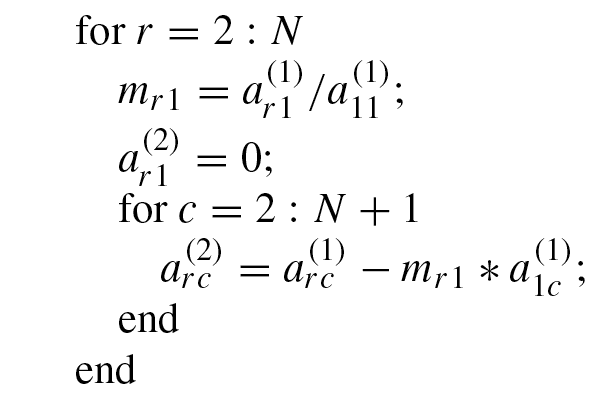
\includegraphics[width=70mm]{chap-2/P49_Step2.png}
\end{center}
\end{figure}
}

\frame{
The new elements are written $a^{(2)}_{r,c}$ to indicate that this is the second time that a number has been stored in the matrix at location $(r,c)$. \\
The result after step 2 is
\begin{equation*}
\left[
\begin{array}{c c c c c | c}
a_{1,1}^{(1)} & a_{1,2}^{(1)} & a_{1,3}^{(1)} & \cdots & a_{1,N}^{(1)} & a_{1,N+1}^{(1)} \\
0                 & a_{2,2}^{(2)} & a_{2,3}^{(2)} & \cdots & a_{2,N}^{(2)} & a_{2,N+1}^{(2)}\\
0                 & a_{3,2}^{(2)} & a_{3,3}^{(2)} & \cdots & a_{3,N}^{(2)} & a_{3,N+1}^{(2)}\\
\vdots        & \vdots        & \vdots        &            & \vdots             & \vdots \\
0                 & a_{N,2}^{(2)} & a_{N,3}^{(2)} & \cdots & a_{N,N}^{(2)} & a_{N,N+1}^{(2)}
\end{array}
\right]
\end{equation*}
}

\frame{
Step $3$ \\
If necessary, switch the second row with some row below it so that $a^{(2)}_{2,2} \ne 0$; then eliminate $x_2$ in rows $3$ through $N$. 
In this process, $m_{r,2}$ is the multiple of row $2$ that is subtracted from row $r$.
\begin{figure}
\begin{center}
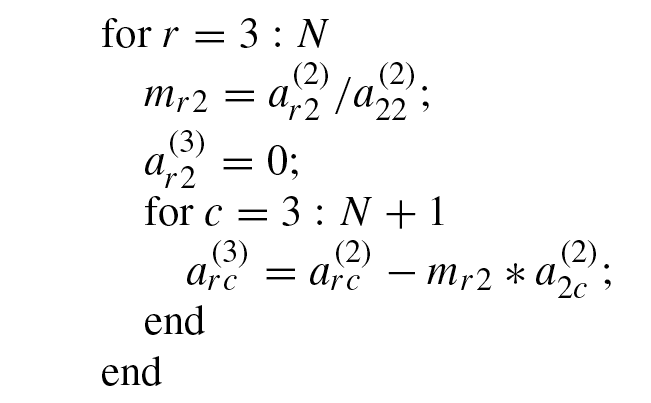
\includegraphics[width=70mm]{chap-2/P50_Step3.png}
\end{center}
\end{figure}
}

\frame{
The new elements are written  $a^{(3)}_{r,c}$ to indicate that this is the third time that a number has been stored in the matrix at location $(r,c)$. \\ 
The result after step 3 is
\begin{equation*}
\left[
\begin{array}{c c c c c | c}
a_{1,1}^{(1)} & a_{1,2}^{(1)} & a_{1,3}^{(1)} & \cdots & a_{1,N}^{(1)} & a_{1,N+1}^{(1)} \\
0                 & a_{2,2}^{(2)} & a_{2,3}^{(2)} & \cdots & a_{2,N}^{(2)} & a_{2,N+1}^{(2)}\\
0                 & 0                 & a_{3,3}^{(3)} & \cdots & a_{3,N}^{(3)} & a_{3,N+1}^{(3)}\\
\vdots        & \vdots        & \vdots        &            & \vdots             & \vdots \\
0                 & 0                & a_{N,3}^{(3)} & \cdots & a_{N,N}^{(3)} & a_{N,N+1}^{(3)}
\end{array}
\right]
\end{equation*}
}

\frame{
Step $p+1$\\
This is the general step. 
If necessary, switch row $p$ with some row beneath it so that $a^{(p)}_{p,p} \ne 0$; then eliminate $x_p$ in rows $p+1$ through $N$. 
Here $m_{r,p}$ is the multiple of row $p$ that is subtracted from row $r$.
\begin{figure}
\begin{center}
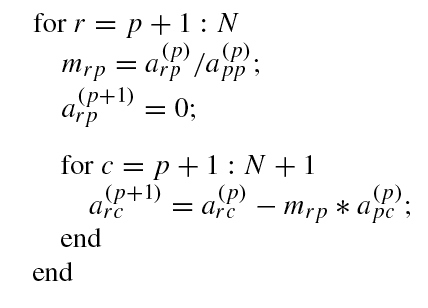
\includegraphics[width=70mm]{chap-2/P51_StepP.png}
\end{center}
\end{figure}
}

\frame{
The final result after $x_{N-1}$ has been eliminated from row $N$ is
\begin{equation*}
\left[
\begin{array}{c c c c c | c}
a_{1,1}^{(1)} & a_{1,2}^{(1)} & a_{1,3}^{(1)} & \cdots & a_{1,N}^{(1)} & a_{1,N+1}^{(1)} \\
0                 & a_{2,2}^{(2)} & a_{2,3}^{(2)} & \cdots & a_{2,N}^{(2)} & a_{2,N+1}^{(2)}\\
0                 & 0                 & a_{3,3}^{(3)} & \cdots & a_{3,N}^{(3)} & a_{3,N+1}^{(3)}\\
\vdots        & \vdots        & \vdots          &            & \vdots             & \vdots \\
0                 & 0                & 0                   & \cdots & a_{N,N}^{(N)} & a_{N,N+1}^{(N)}
\end{array}
\right]
\end{equation*}
The {\Large upper-triangularization} process is now complete.
\begin{itemize}
\item Since $A$ is nonsingular\footnote{非奇异的,满秩}, when row operations are performed the successive matrices are also nonsingular. 
\item This guarantees that $a^{(k)}_{k, k} = 0$ for all $k$ in the construction process.
\item Hence back substitution can be used to solve $U X = Y$ for $X$, and the theorem is proved.
\end{itemize}
}

\frame{
\begin{block}{Pivoting to Avoid $a_{pp}^{(p)} = 0$}
\begin{itemize}
\item If $a_{pp}^{(p)} = 0$, row $p$ cannot be used to eliminate the elements in column $p$ below the main diagonal. 
\item It is necessary to find row $k$, where $a_{pp}^{(p)} \neq 0$ and $k > p$, and then interchange row $p$ and row $k$ so that a nonzero pivot element is obtained. 
This process is called pivoting, and the criterion for deciding which row to choose is called a pivoting strategy.
\end{itemize}
\end{block}
\begin{block}{The trivial pivoting strategy is as follows.} 
\begin{itemize}
\item If $a_{pp}^{(p)} \neq 0$, do not switch rows. 
\item If $a_{pp}^{(p)} = 0$, locate the first row below $p$ in which $a_{pp}^{(p)} \neq 0$ and switch rows $k$ and $p$. 
\item This will result in a new element $a_{pp}^{(p)} \neq 0$, which is a nonzero pivot element. 
\end{itemize}
\end{block}
}


\frame{
\frametitle{Example.}
\begin{block}{}
\begin{itemize}
\item (a) Use MATLAB to construct the augmented matrix for the linear system in the above Example; 
\vspace{3mm}
\item (b) use the max command to find the element of greatest magnitude in the first column of the coefficient matrix $A$; 
\vspace{3mm}
\item and (c) break the augmented matrix in (1.22) into the coefficient matrix $U$ and constant matrix $Y$ of the upper-triangular system $UX = Y$. 
\end{itemize}
\end{block}
}

\frame{
\frametitle{Example (a)}
%\begin{verbatim}
>> A=[1 2 14; 2  4 3;4 2 2 1; -3 13 2]; \\
>> B=[13 28 20 6]';  \\
>>Aug=[A B] \\
Aug= \\
1 2 1 4 13\\ 
2 0 4 3 28 \\
4 2 2 1 20 \\
-3 1 3 2 6 
%\end{verbatim}
}

\frame{
\frametitle{Example (b)} 
In the following MATLAB display, a is the element of greatest magnitude in the first column of $A$ and $j$ is the row number. \\
%\begin{verbatim}
>>[a,j ]=max(abs(A(1:4,l))) \\
a= \\
4 \\
j= \\
3 
%\end{verbatim}
}

\frame{
\frametitle{Example (c)} 
Let $Augup = [U | Y]$ be the upper-triangular matrix.\\
%\begin{verbatim}
>> Augup=[1 2 1 4 13; 0 -4 2 -5 2; 0 0 -5 -7.5 -35; a a 0 -9 -18]; \\
>> U=Augup(I:4,1:4) \\
U= \\
1. 0000  2.0000    1.0000    -4.0000 \\
0            -4.0000  2.0000    -5.0000 \\
0           0              -5.0000  -7.5000 \\
0           0              0             -9.0000 \\
>> Y=Augup(1:4,5)\\
Y= \\
13 \\
2 \\
-35 \\ 
-18 
%\end{verbatim}
}

